\documentclass{ubicomp2012}
\usepackage{times}
\usepackage{url}
\usepackage{graphics}
\usepackage{color}
\usepackage[pdftex]{hyperref}
\hypersetup{%
pdftitle={iPlant}, pdfauthor={Jesper Sandberg and Thomas Kokholm}, pdfkeywords={iPlant, Inteligent Plant System, Pervasive, Arduino}, bookmarksnumbered, pdfstartview={FitH}, colorlinks,
citecolor=black, filecolor=black, linkcolor=black, urlcolor=black,
breaklinks=true, }
\newcommand{\comment}[1]{}
\definecolor{Orange}{rgb}{1,0.5,0}
\newcommand{\todo}[1]{\textsf{\textbf{\textcolor{Orange}{[[#1]]}}}}

%\pagenumbering{arabic}  % Arabic page numbers for submission.  Remove this line to eliminate page numbers for the camera ready copy

\begin{document}
% to make various LaTeX processors do the right thing with page size
\special{papersize=8.5in,11in}
\setlength{\paperheight}{11in}
\setlength{\paperwidth}{8.5in}
\setlength{\pdfpageheight}{\paperheight}
\setlength{\pdfpagewidth}{\paperwidth}

% use this command to override the default ACM copyright statement
% (e.g. for preprints). Remove for camera ready copy.
\toappear{Report written at the IT-University of Copenhagen for the course Pervasive Project Fall 2012. The copyright remains with the authors.}



\title{iPlant: Inteligent Plant System}
\subtitle{SPCL-2012 - Report Synopsis}
\numberofauthors{2}
\author{
  \alignauthor Jesper Sandberg\\
    \affaddr{IT University of Copenhagen}\\
    \affaddr{Rued Langgaardsvej Vej 7}\\
    \affaddr{DK-2300 Copenhagen S}\\
    \email{jesan@itu.dk}
 \alignauthor Thomas Kokholm\\
    \affaddr{IT University of Copenhagen}\\
    \affaddr{Rued Langgaardsvej Vej 7}\\
    \affaddr{DK-2300 Copenhagen S}\\
    \email{tkok@itu.dk}  }
\maketitle

\section{ABSTRACT}
People enjoy plants, their benefits and the feeling related to nurturing them. However for most people it becomes challenging to keep them healthy and alive. To accommodate this challenge we have developed a prototype, which makes a plant more self-sufficient, watering itself from a large water tank and providing itself with artificial sunlight.
The prototype reports status of its current conditions and also reminds the user to refill the water tank.
Through this prototype we hope that people will enjoy having plants without the challenges related to absent or forgetfulness.

\section{AUTHOR KEYWORDS}
Plant monitoring, Automatic watering, Artificial sunlight, Wi-Fi Communication

\section{ACM CLASSIFICATION KEYWORDS}
Arduino, RHT03, Drip irrigation, Wi-Fi

\section{INTRODUCTION}
Since the dawn of time humans has lived and enjoyed the beauty and benefits \cite{The-Benefits-of-Plants-and-Landscaping, houseplants-make-you-smarter, People-Plant-Relationship} of household plants. However since then, the way of nurturing plants almost haven't evolved. In a household plants are grown in mold or dirt, potted and placed on the windowsill. Due to this plants are dependent on regular nurturing - watering them and providing the right amount of sunlight to stay alive and grow.

This has resulted in a number of challenges. People often forget to nurture their plant(s)[0 questionnaire], between daily activities. The result is often that plants suffer and die, gets discarded and simple replaced by a new one \cite{Danes-spend-approx-2000-a-year-on-plants}, or people stop having plants altogether [0 questionnaire and maybe interview]. This issue have even gotten as far as creating a successful industry for artificial/non-living plants made out of plastic.
People often develop a strong affection towards their plants. A relationship build on regular caretaking in order to grow and evolve - similar like animal and humans grow and evolve in life\cite{People-Plant-Relationship}. Research has shown that there is a link between nurturing plants as well as children, and how children treats nature as an adult\cite{Childrens-Active-and-Passive-Interactions-with-Plants}.

In order to solve all or at least many of the above issues, engineers try to create helpful systems that keep plants alive by i.e. automatic watering [0 related work] or reminders [0 related work]. However these systems do not solve the overall challenges. Plants still need humans as caretakers - one way or the other. So how can we solve all these issues, with forgetful humans, plants that require water and sunlight, as well as keeping the relationship between plant and people? Based on the above context, we believe there is a need for a home gardening system, which take care of all the different aspects in nurturing plants.

In this paper we explain how our system works as well as how it solves the above issues, we back up our theory of this system, by completing test scenarios on how well the system is able to perform in both a tough environment as well as a test in a real scenario environment. Based on the description of our system, our qualitative and quantitative research combined with our test scenarios we have drawn conclusions in order to show what we have achieved \{add more once we have finished the conclusion\}. Overall we hope that this research will contribute to more people having the benefits of plants, as well as contributing to the advancement for people homes of the future, e.g. home automation.

Futhermore we expect our prototype and research to shows that automation doesn't necessarily remove or destroy the phycologial aspects of caretaking plants. Iplant is intended to be helpfull, assistive and smart.

\section{RELATED WORK}
Make-Digital magazine posted a guide on microcontroller-assisted gardening\cite{how-to-make-a-gardening-system}, using an Arduino microprocessor, fluorescent light, a submersible water pump and 1" galvanized nails.

\begin{figure}[h!]
\centering
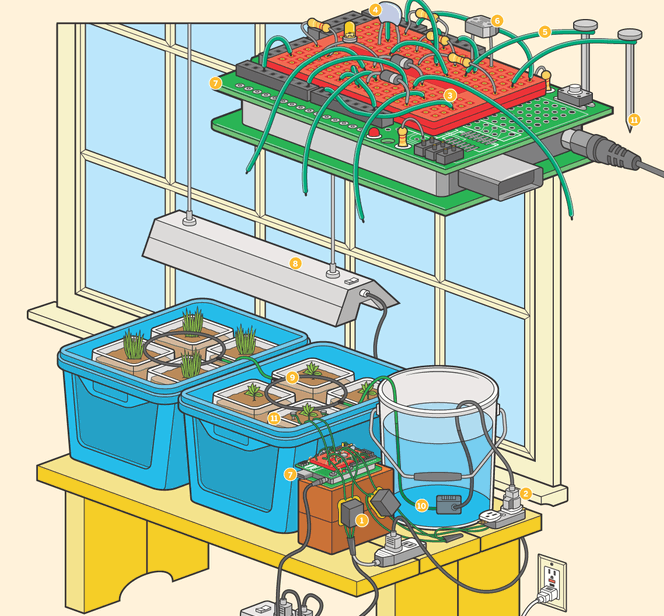
\includegraphics[width=\columnwidth]{howto-gardening.png}
\caption{Illustrating the scale and complexness of a "do-it-yourself" guide on microcontroller-assisted gardening. Image: Make-Digital Magazine.}
\label{fig:MakeDigitalMagazine}
\end{figure}

This system relates much to our idea, but the focus in their guide is "only" on automation. Further more this gardening system is based heavily on a "do-it-yourself" concept. Our idea is opposite: designing a finished solution, that is less demanding, and easy to use.
The scale of the MakeDigital solution is also very large, whereas our solution is small and compact. Even further, the Make-digital solution is highly complex to install, with lots of wiring and tubes going from bucket to bucket. See figure ~\ref{fig:MakeDigitalMagazine}

In our research, we discovered that almost every solution requires large implementations, much wiring and setup. The solutions on the market today aren't portable, and they tend to take up a large amount of space. They relate more to greenhouse-installations than regular household plants.

Our solution/implementation focus on household plants and is intended to replace regular pots, without being large- or bulky installations. The user's focus should remain on keeping plants - not on the technological and mechanical parts behind, in contrary to the make-digital's how-to guide.

Our system will be assistive but not dominating. In contrast to other solution the user is still capable of watering the plant himself without it affecting our system.

Very few commercial gardening systems (intended for home usage) fully attend a plant’s needs. Most systems are based on watering "only". Popular products like: Self Watering Probes \cite{self-watering-probes} and Drip Irrigation Systems \cite{moreland} simply pump water from an external bucket, controlled by timer intervals.
It is difficult to find a home gardening system that handles both watering and sunlight. It is even more difficult to purchase a system, that use humidity to determine a plants actual requirements.


\begin{table*}
\begin{center}
\renewcommand{\arraystretch}{1.5}
%\begin{tabular}{| p{2.5cm} | p{1cm} | p{1cm} | p{1cm} | p{1cm} |}
\begin{tabular}{| p{7cm} | p{2cm} |p{2.5cm}  | p{2cm} | p{2cm} |}
\hline
                                                    & Timer                        & Moisture Sensor                        & Portable  & Interactive \\ \hline
        Moreland AWS-10                             & Yes                          & ~                                      & No        & No        \\ \hline
        Indoor / Outdoor Moisture Sensor Meter      & Yes                          & Yes                                    & No        & No         \\ \hline
        Easy2Grow Autopots                          & Yes                          & ~                                      & No        & No         \\ \hline
        Moisture Matic Automatic Watering System    & Yes                          & ~                                      & No        & No         \\ \hline
        CobraCo Plant Sitter Water System           & Yes                          & ~                                      & No        & No         \\ \hline
        Oasis Indoor Automatic Drip Watering System & Yes                          & ~                                      & No        & No         \\ \hline
        Self Watering Probes                        & Yes                          & No                                     & Yes       & No         \\ \hline
        System 8                                    & Yes                          & ~                                      & No        & No         \\ \hline
        iPlant                                      & No                           & Yes                                    & Yes       & Yes (Web+Email)      \\ \hline
\end{tabular}
\caption{Comparing the different features of various home gardening systems.}
\label{tab:Comparison Table}
\end{center}
\end{table*}


\section{BACKGROUND AND RESEARCH METHOD}
Explain why we want to develop this project and what we have done in order to succeed in doing it.

\subsection{Background and Motivation}
For years we have enjoyed the beauty and benefit of green plants. Yet people often struggle to keep their plants alive and fit. Plants require much attention with regular watering \& sunlight - easily forgotten in daily activities.

However plants are important for a healthy environment while they contribute to clean and natural air with the production of oxygen.
They help convert CO2 gasses and neutralize toxins in the air. \cite{naturstyrelsen}

Our automatic gardening system: iPlant will help attend plant(s) and provide users with information on temperature, humidity and general air quality near their plant(s). Using iPlant people can engage in having many different plants with absolute minimum effort. Even plants that require much attention like i.e. orchidaceae which are otherwise difficult to keep[1].

Furthermore users can combine multiple plants and monitor an entire villa or i.e. an office location with plants in different rooms connected to a local Wi-Fi network. This ensures a natural work environment and provides all the information about the plant(s) accessible from the internet.

\subsection{Idea}
The main idea is to create a system that is capable of both watering and illuminate the plant(s). The system should be intelligent and capable of notifying the owner of the plant(s) with status information obtained through sensors placed directly within each plant.

Multiple plants can be connected to a local network using Wi-Fi and monitored from a web interface.

Potting a plant combined with our solution provides the plant with the necessary attention for it to sustain on its own for longer periods of time, even when located with no access to sunlight. Our solution will automatically water the plant regularly - keeping a fixed level of humidity in the soil.

Focus is on developing a prototype that is:
\begin{itemize}
    \item Small in scale
    \item Easy to use (and deploy)
    \item Ready from the beginning
\end{itemize}

iPlant should resemble regular household pots, yet packet with technology, assisting people in nurturing their plant(s).

\subsection{Scenario}
A family leaves their home for two weeks of much needed vacation. During their stay, their plants suffer from their absence.
In one room the curtains are closed, and prevent the plants from obtaining sufficient sunlight - they stop growing and begin to wither and may die.
In another room plants are over-watered in the hope that they will survive during the absence. They unfortunately drown from the massive watering.
In a third room the family did not water their plants sufficiently and wither from regular exposure to sunlight without moist soil to drain from.

If only there was a system which could attend these plants, then the family would not only continue to have their plants upon return, they wouldn't ever have to worry when leaving home.

\section{Plant Management System}
An intelligent plant system denoted iPlant, which helps users attend plant(s). A concept based on automatic watering, artificial sunlight combined and with sensors for monitoring.
iPlant is a step towards more modern homes, automatic homes, which takes care of itself via many sensors and small computers. Thereby giving more time to the home owners for doing what they actually want to do.
The iPlant system includes the option to disable the automatic part of the system and therefore only have the monitoring, this allows some humans, which prefer to take care of the plant on their own, to continue doing so, but with the benefit of getting messages from their plant about its current status.[0]

\subsection{Relation Aspect}
\{Reference to the introduction part\}
In order to try to compensate for some of these issues, we have developed a feedback feature to our plant management system, note that this feedback is customizable, so that users can receive e-mails from the plant, telling them about how they are doing. These messages will not simply be "hard data", but be structured in a way so that the plant is speaking and maybe even joking about its condition and what is currently going on in “its life".

The iPlant system will have the ability to entirely disable automatic parts, so that only the monitoring part maintain active. This will ensure maximum satisfaction for all users.



\section{EVALUATION \& RESULTS}
\subsection{Test Settings}
\subsubsection{Stress Test}
Explain our basement (strength) test, which consists of testing out the watering and UV diode system in a dark basement over a time period of at least 3 weeks.
Explain the challenges and results of this test, as well as why our various results are as they are.

\subsubsection{Human Tnteraction test}

Write about our human interaction test, which is testing our system in a real scenario in a home with humans not related to the project - nurturing the iPlant.
Explain the different challenges and results of this test, focus on the human aspect. How the plant is perceived, refer to interview(s) with the humans from our test scenario.
Answer:
+ Can it work? and if not why?
+ Does it become more boring to have plants?

 this is a longitudunal study- We do it because our user need long time to test/try out our solution
    write what a longitudinal is and the problems about having a long test time (plant grow slow)

simulte the finished beutiful system. Where would people place the plants. What problem arise and etc. Even without the system working but fake it!

\section{DISCUSSION}
Discuss the challenges of our system, with high regard to our evaluation and results. Also discuss and evaluate the future use, work and applications for our iPlant.

\section{CONCLUSION}
Draw conclusions from what is written in the above sections.

\section{ACKNOWLEDGEMENTS}
Give acknowledgements to supervisors(Thomas, Shahram), people who helped us (Sebastian, people we interviewed etc.), organizations which have been of assistance (plant nursery, ITU, our workplace, etc.).

\subsection{Supervisor}
Sebastian B\"uttrich\\
IT University of Copenhagen\\
Rued Langgaardsvej Vej 7\\
DK-2300 Copenhagen S\\
sebastian@itu.dk


\vfill\eject


\bibliographystyle{abbrv}
\bibliography{sample}

\end{document}


